\chapter{Analiti"cna izpeljava vplivov dinami"cne in stati"cne ekscentri"cnosti}

V tem poglavju bom analiti"cno prikazati vpliv napak omenjenih ekscentri"cnosti, ki se pojavita zaradi neprimerne vgradnje te vrste enkoderja. Napaki razli"cno vplivati na izhode senzorja, zato ju lahko obravnamvam posami"cno. Preko analiti"cne izpeljave bomo spoznali kako se spreminja lokacija Hall-ove sonde glede na magnet ob pravilni monta"zi. Z vpeljavo dodane ekscentri"cnosti v model bomo videli, kako se trajektorija gibanja Hall-ove sonde glede na magnet spremeni. S poznavanjem lokacije Hall-ove sonde nad magnetom bomo lahko od"citali vrednost \Bz.


\section{Definicija koordinatnih sistemov}

Definirajmo kartezi"cni koordinatni sistem, ki ima v izhodi"scu postavljen radialno magnetiziran magnet. Na poljubno to"cko $S_{h0}(x_0,y_0)$, vendar ne v izhodi"s"ce postavimo Hall-ovo sondo. Na sliki \ref{fig:def_kks} je prikazan tak sistem. Hall-ova sonda je postavljena na abcisno os za la"zje razumevanje. Vrednost $y_0$ je lahko poljubna in kon"cna re"sitev izpeljave bo splo"sna za poljubno lokacijo Hall-ove sonde v za"cetni legi.

\begin{figure}[h!]
	\centering
	\begin{tikzpicture}
	\magnet {0} {0} {0}{$S_r(0, 0)$}{1};
	\hall {2.3}{0} {0};
	\end{tikzpicture}
	\caption{Definicija koordinatnega sistema z magnetom in Hall-ovo sondo}
	\label{fig:def_kks}
\end{figure}

Z rotacijo magneta za kot $\theta$, se lokacija Hall-ove sonde glede na magnet spremeni. Nova lokacija Hall-ove sonde glede na magnet je enaka, "ce namesto magnet, zarotiramo Hall-ovo sondo za kot $-\theta$ . Novo lokacjo Hall-ove sonde glede na magnet lahko zapi"semo z rotacijsko matriko.

\begin{equation}
\label{equ:rotacija_hall}
\begin{bmatrix} x\\y \end{bmatrix}=
\begin{bmatrix} \cos(-\theta)&-\sin(-\theta)\\\sin(-\theta)&\cos(-\theta) \end{bmatrix}
\begin{bmatrix} x_0\\y_0 \end{bmatrix}
\end{equation}

Argument rotacijske matrike je $-\theta$, pri "cemer vemo, da smo namesto magneta zarotirali Hall-ovo sondo v nasprotno smer. Z upo"stevanjem lihosti funkcije sinus in sodosti funkcije kosinus, se ena"cba \ref{equ:rotacija_hall} poenostavi v:
\begin{equation}
\label{equ:rotacija_hall_simplify}
\begin{bmatrix} x\\y \end{bmatrix}=
\begin{bmatrix} \cos(\theta)&\sin(\theta)\\-\sin(\theta)&\cos(\theta) \end{bmatrix}
\begin{bmatrix} x_0\\y_0 \end{bmatrix}
\end{equation}




\begin{figure}[h!]
%	\centering


    \begin{subfigure}[b]{0.5\textwidth}
	\centering
	
		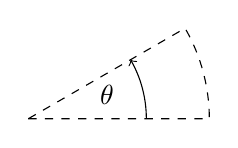
\begin{tikzpicture}
		[scale=1, every node/.style={scale=1}]
				\magnet {0} {0} {30}{}{1}
				\hall {2.3}{0} {0};
				\draw [dashed](0,0)--(2.3,0) arc (0:30:2.3)--(0,0);
				\node at(1,0.3){$\theta$};
                \draw [->] (1.5,0) arc (0:30:1.5);
		\end{tikzpicture}
	\caption{Zasukan magnet za kot $\mathrm{\theta}$}
	\label{subfig:zasuk_magnet}
\end{subfigure}
\begin{subfigure}[b]{0.5\textwidth}
	\centering
	
		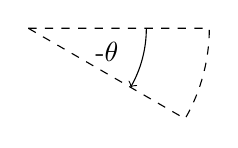
\begin{tikzpicture}[scale=1, every node/.style={scale=1}]		
				\magnet {0} {0} {0}{}{1}
				\hall {1.99}{-1.15} {-30};
				\draw [dashed](0,0)--(2.3,0) arc (0:-30:2.3)--(0,0);
				\node at(1,-0.3){-$\theta$};
                \draw [->] (1.5,0) arc (0:-30:1.5);
		\end{tikzpicture}
	
	\caption{Zasukan senzor za kot $\mathrm{-\theta}$}
	\label{subfig:zasuk_hall}
\end{subfigure}

\caption{Sprememba lokacije glede na magnet ob rotaciji}
\label{fig:zasuk_magneta}

\end{figure}



\section{Izpeljava gibanja lokacije Hall-ove sonde na magnet pri dinami"cni ekscentri"cnosti}

Opazujmo sedaj sistem gibanja Hall-ove sonde glede na magnet ter dinami"cno ekscentri"cnost. Magnet je
 postavljen v izhodi"sce koordinatnega sistema $S_m(0,0)$. Sedaj magnet izmaknemo v novo lego $S_{m1}(\Delta
  x_d,\Delta y_d)$ (Slika \ref{fig:def_din_eks}). Os vrtenja je "se vedno postavljena v izhodi"s"ce
   koordinatnega sistema. Sredi"sce magneta $S_{m1}(\Delta x_d,\Delta y_d)$ tako tekom vrtenja okoli
    koordinatnega izhodi"sca opi"se kro"znico z radijem $\sqrt{\Delta x_d^2+\Delta y_d^2}$. V sistem sedaj
     dodajmo Hall-ovo sondo v njeno za"cetno lego glede na izhodi"sce $S_{h0}(x_0,y_0)$.




\begin{figure}[h!]
	\centering
	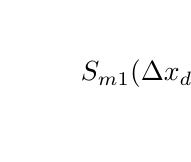
\begin{tikzpicture}
		\magnet {0.6} {0.3} {0}{$S_{m1}(\Delta x_d,\Delta y_d)$}{1};
		\draw [dashed]  (0,0) circle (0.67);
		\draw (0,0)--(0.6,0.3);
		\fill (0,0) circle [radius=1pt];
		\node at (0.35,-0.3){$S_0(0,0)$};
		\hall {2.3}{0} {0};
		\kks{3}
	\end{tikzpicture}
	\caption{Shema definicije dinami"cne ekscentri"cnosti vpliva na magnet}
	\label{fig:def_din_eks}
\end{figure}




Enako gibanje Hall-ove sonde na magnet lahko dose"zemo tudi z obrnjenim sistemom. Vrnimo magnet v izhodi"s"cno lego $S_m(0,0)$. Sedaj postavimo os vrtenja magneta v to"cko $(-\Delta x_d,-\Delta y_d)$. Hall-ovo sondo postavimo v to"cko $S_{h1}(x_0-\Delta x_d,y_0 - \Delta y_d).$



\begin{figure}[h!]
	\centering
	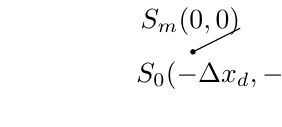
\begin{tikzpicture}
		\magnet {0} {0} {0}{$S_{m}(0,0)$}{1};
		\draw (0,0)--(-0.6,-0.3);
		\fill (-0.6,-0.3) circle [radius=1pt];
		\node at (0,-0.6){$S_0(-\Delta x_d,-\Delta y_d)$};
		\hall {1.7}{-0.3} {0};
		\kks{3}
	\end{tikzpicture}
	\caption{Shema definicije dinami"cne ekscentri"cnosti vpliva na Hall-ovo sondo}
	\label{fig:def_din_eks_na_stator}
\end{figure}

Sistema prikazana na slikah \ref{fig:def_din_eks} in \ref{fig:def_din_eks_na_stator}, se v za"cetnih legah ne razlikujeta. Sedaj zarotirajmo Hall-ovo sondo okoli osi vrtenja $S_0(-\Delta x_d,-\Delta y_d)$. Hall-ova sonda se giblje glede na magnet enako, kot "ce bi magnet zavrteli z dinami"cno ekscentri"cnostjo (Slika \ref{fig:def_din_eks}). Gibanje Hall-ove sonde na magnet je izra"zeno kot gibanje po kro"znici s sredi"s"cem v to"cki $(-\Delta x_d,-\Delta y_d)$.

\begin{figure}[h!]
	\centering
	\begin{tikzpicture}
		\magnet {0} {0} {0}{}{1};
		\draw [dotted]  (-0.6,-0.3) circle (2.3);
		\draw (0,0)--(-0.6,-0.3);
		\fill (-0.6,-0.3) circle [radius=1pt];
		\hall {1.39}{-1.45} {-30};
		\draw [dashed](-0.6,-0.3)--(1.7,-0.3) arc(0:-30:2.3)--(-0.6,-0.3);
		\node at(0.4,-0.6){$-\theta$};
        \draw [->] (0.9,-0.3) arc (0:-30:1.5);
		\kks{3}
	\end{tikzpicture}
	\caption{Potek Hall-ove sonde ob rotaciji glede na magnet ob dinami"cni ekscentri"cnosti}
	\label{fig:potek_sonde_din_eks}
\end{figure}

Potek Hall-ove sonde ob rotaciji z upo"stevanjem dinami"cne ekscentri"cnosti lahko zapi"semo kot (\ref{equ:rotacija_hall_simplify}) z dodatkom enosmerne komponente dinami"cne ekscentri"cnosti.

\begin{equation}
\label{equ:rotacija_hall_din}
\begin{bmatrix} x\\y \end{bmatrix}=
\begin{bmatrix} \cos(\theta)&\sin(\theta)\\-\sin(\theta)&\cos(\theta) \end{bmatrix}
\begin{bmatrix} x_0\\y_0 \end{bmatrix}
+
\begin{bmatrix} -\Delta x_d\\-\Delta y_d \end{bmatrix}
\end{equation}

V (\ref{equ:rotacija_hall_din}) lahko izrazimo - in izraz se poenostavi.

\begin{equation}
\label{equ:rotacija_hall_din_simplify}
\begin{bmatrix} x\\y \end{bmatrix}=
\begin{bmatrix} \cos(\theta)&-\sin(\theta)\\\sin(\theta)&\cos(\theta) \end{bmatrix}
\begin{bmatrix} x_0\\y_0 \end{bmatrix}
-
\begin{bmatrix} \Delta x_d\\\Delta y_d \end{bmatrix}
\end{equation}

\section{Izpeljava gibanja lokacije Hall-ove sonde na magnet pri stati"cni ekscentri"cnosti}


Postavimo sistem nazaj v izhodi"scno lego, brez ekscentri"cnosti. Tako sredisce magneta, kot os vrtenja postavimo v izhodi"sce. Hall-ova sonda je postavljena v to"cko $S_{h0}(x_0,y_0)$. Sedaj premaknimo Hall-ovo sondo za $(\Delta x_s, \Delta y_s)$, v novo to"cko $S_{h1}(x_0+\Delta x_s, y_0+\Delta y_s)$. Na sliki \ref{fig:def_sta_eks} je prikazana le stati"cna ekscentri"cnost v y-osi, vendar celotni razmislek velja za obe stati"cni ekscentri"cnosti enako.


\begin{figure}[h!]
	\centering
	\begin{tikzpicture}
	\magnet {0} {0} {0}{}{1};
	\hall {2.4}{-0.6} {0};
	\draw[<->,dotted] (0,0)--(0,-0.6);
	\draw[dotted] (2.3,-0.6)--(0,-0.6);
	\node at (0.4,-0.3){$\Delta y_s$};
	\end{tikzpicture}
	\caption{Shema definicije stati"cne ekscentri"cnosti}
	\label{fig:def_sta_eks}
\end{figure}

Po enakem razmi"sljanju kot v zgornjih poglavjih, sedaj zarotirajmo Hall-ovo sondo za kot \kol{-\theta} okoli izhodi"s"ca. Hall-ova sonda se giblje po kro"znici z radijem $\sqrt{(x_0+\Delta x_s)^2+(y_0+\Delta y_s)^2}$.


\begin{figure}[h!]
	\centering
	\begin{tikzpicture}
	\magnet {0} {0} {0}{}{1};
	\hall {1.69}{-1.67} {-30};
	\draw[<->,dotted] (0,0)--(-0.3,-0.52);
	\draw[dotted] (1.69,-1.67)--(-0.3,-0.52);
	\draw [dashed] (0,0) -- (2.377,0) arc(0:-30:2.377)--(0,0);
	\node at (0.8,-0.2) {\kol{-\theta}};
	\draw [dotted] (0,0)circle[radius=2.377];
%    \draw [dotted, <->] (0,0)--(2.06,1.19);
%    \node at (4.03,0.6){$\sqrt{(x_0+\Delta x_s)^2+(y_0+\Delta y_s)^2}$};
	\draw [dotted, <->] (0,0)--(1.69,-1.67);
    \draw [->] (1.5,0) arc (0:-30:1.5);
	\end{tikzpicture}
	\caption{Potek Hall-ove sonde ob rotaciji glede na magnet ob stati"cni ekscentri"cnosti}
	\label{fig:def_sta_eks_stat}
\end{figure}


To lahko zapi"semo v izraz (\ref{equ:rotacija_hall_simplify}) kot:

\begin{equation}
\label{equ:rotacija_hall_stat}
\begin{bmatrix} x\\y \end{bmatrix}=
\begin{bmatrix} \cos(\theta)&\sin(\theta)\\-\sin(\theta)&\cos(\theta) \end{bmatrix}
\begin{bmatrix} x_0+\Delta x_s\\y_0+\Delta y_s \end{bmatrix}
\end{equation}







\section{Kon"cna ena"cba za dolo"canje lokacije Hall-ove sonde}

Do sedaj smo postopoma izpeljali ena"cbe za:
\begin{itemize}
  \item sistem magneta in Hall-ove sonde ob pravilni monta"zi
  \item sistem magneta in Hall-ove sonde z dinami"cno ekscentri"cnostjo magneta
  \item sistem magneta in Hall-ove sonde z stati"cno ekscentri"cnostjo Hall-ove sonde
\end{itemize}

Ena"cbi sistema z ekscentri"cnostjo sti med seboj neodvisni zato lahko ena"cbe sistemov zdru"zimo. Uporabimo princip superpozicije in dobimo kon"cno ena"cbo za lociranje Hall-ove sonde glede na magnet v odvistnosti od zasuka magneta, z upo"stevanjem vpliva tako dinami"cne kot stati"cne ekscentri"cnosti. Kon"cna ena"cba se glasi:

\begin{equation}
\label{equ:rotacija_hall_koncna}
\begin{bmatrix} x\\y \end{bmatrix}=
\begin{bmatrix} \cos(\theta)&\sin(\theta)\\-\sin(\theta)&\cos(\theta) \end{bmatrix}
\begin{bmatrix} x_0+\Delta x_s\\y_0+\Delta y_s \end{bmatrix}-
\begin{bmatrix} \Delta x_d\\\Delta y_d \end{bmatrix}
\end{equation}


Ogledali smo si, kako je ob rotaciji locirana Hall-ova sonda glede na magnet. Ogledali smo si tudi, kako na lokacijo sonde vplivati dinami"cna in stati"cna ekscentri"cnost. S poznavanjem magnetnega polje $B_z=B_z(x , y)$, lahko dolo"cimo kak"sno vrendost polja $B_z$ pomeri Hall-ova sonda ob rotaciji ($B_z=B_z(\theta)$). Ob poznavanju polja $B_z$, lahko dolo"cimo zasuk magneta glede na postavitev Hallove sonde.


\chapter{Izpeljava poteka polja $B_z(\theta)$ in ocena napake zaradi ekscentri"cnosti}

V tem poglavju si bomo ogledali kak"snomagnetno polje  pomeri Hall-ova sonda. Ogledali si bomo magnet, ter kako senzor RM44 meri magnetno polje. Preko pomirjenega polja, bomo izra"cunali kak"sna je napake pomerjenega kota od referen"cnega in kako se napaka spreminja z ekscentri"cnostjo.

\section{Definicija  gostote magnetnega polja $B_z$}

Predlagan magnet s strani proizvajalca senzorja je radialno magnetiziran s premerom 4 mm.
Dajalnik pozicije RM44 meri Z-komponento gostote magnetnega polja zato se lahko osredoto"cimo le nanjo citeAM8192. Potek komponente $B_z$ nad cilindri"cnim magnetom je prikazan na sliki \ref{fig:magnetno_polje}.

%Magsnetno polje  v prostoru lahko izra"cunamo z Biot-Savartovim zakonom. Poznati moramo specifikacije trajnega magneta in izra"cunati integral po prostoru. Tako dobimo v poljubni to"cki v prostoru vrednost B.  Hall-ove sonde v senzorju RM44 merijo le z-komponento magnetnega polja, zato se lahko osredoto"cimo le nanjo. Odvistnost z-komponente vektorja B na konstantni vi"sini od magneta je vidno na sliki \ref{fig:magnetno_polje}.



\begin{figure}[h]
	\centering
		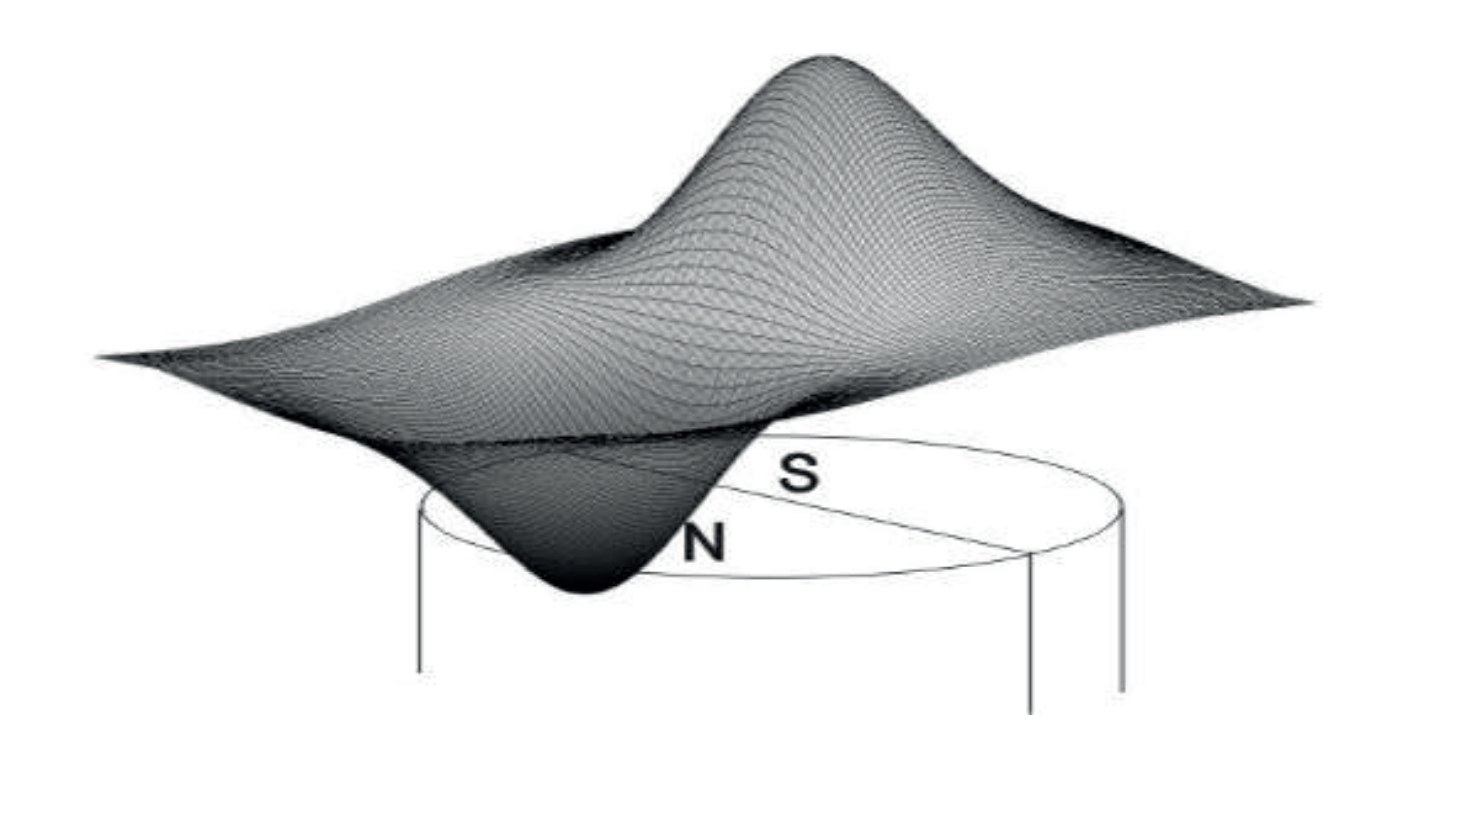
\includegraphics[width=0.75\columnwidth]{./Slike/magnetno_polje.jpg}
	\caption{z-komponenta vektorja gostote magnetnega polja nad cilindri"cnim magnetom citeAM8192}
	\label{fig:magnetno_polje}
\end{figure}


Potek z-komponente lahko izra"cunamo po Biot-Savartovim zakonom oz. numeri"cno se"stejemo prispevke posameznih del"ckov magneta. Tako dobimo vrednost celotnega vektorja gostote magnetnga polja v posamezni to"cki. Magnetno polje z komponente v okolici osi vrtenja magneta lahko aproksimiramo z ravnino

\begin{equation}
\label{equ:poljeB}
B_z(x,y)=k\cdot x.
\end{equation}

Tak"sna aproksimacija zadostuje za ocenitev poteka napake. S poznavanjem lokacije Hall-ove sonde, kar smo si ogledali v prej"snjem poglavju, sedaj dobimo potek pomerjene komponente gostote magnetnega polja. Aprokisirano polje je linearno odvisno od x komponente. Za la"zje razumevanje definirajmo konstanto $k$ enako 1.

\section{Postavitev Hall-ovih sond za zajem polja in pomerjeno polje v odvistnosti od ekscentri"cnosti}
Sedaj si oglejmo, kako bi dolo"cili kot zasuka poljubne to"cke okoli izhodi"s"ca. Definirajmo kartezi"cni koordinatni sistem, in v njem poljubno to"cko $(x_0,y_0)$, ki ni v izhodi"s"cu(Slika \ref{fig:dolocitev_kota}).
Za dolo"canje kota $\varphi$ je potrebno poznati poznati polo"zaj to"cke. Kot $\varphi$ dolo"cimo preko trigonometri"cne funkcije $\arctan$: $$\varphi=\arctan\frac{y_0}{x_0}$$



\begin{figure}[h!]
	\centering
	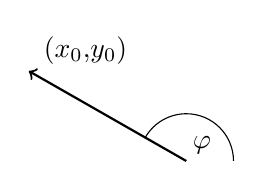
\begin{tikzpicture}[scale=4]
	\CaCS{0.75}{0}{0}
	\draw [->,thick](0,0)--(-0.5,0.2855);
	\draw (0.15,0) arc (0:150:0.15);
	\node at (0.05,0.05){$\varphi$};
%	\node at (-0.5,0.285) {\textbullet};
	\node at (-0.32,0.35) {($x_0$,$y_0$)};
	\end{tikzpicture}
	\caption{Slika za pomo"c pri dolo"canju kota}
	\label{fig:dolocitev_kota}
\end{figure}


Za dolo"citev kota $\varphi$  je dovolj poznati "ze projekciji vektorja na koordinatni osi(slika \ref{fig:dolocitev_kota_2}),

\begin{figure}[h!]
	\centering
	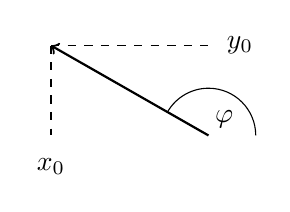
\begin{tikzpicture}[scale=4]
	\CaCS{0.75}{0}{0}
	\draw [->,thick](0,0)--(-0.5,0.2855);
	\draw (0.15,0) arc (0:150:0.15);
	\node at (0.05,0.05){$\varphi$};
	\draw [dashed] (-0.5,0.2855)--(-0.5,0);
	\draw [dashed] (-0.5,0.2855)--(0,0.2855);
	%	\node at (-0.5,0.285) {\textbullet};
%	\node at (-0.32,0.35) {($x_0$,$y_0$)};
	\node at(-0.5,-0.1){$x_0$} ;
	\node at(0.1,0.2855){$y_0$};
	\end{tikzpicture}
	\caption{Slika za pomo"c pri dolo"canju kota}
	\label{fig:dolocitev_kota_2}
\end{figure}


"Ce poznamo projekciji to"cke na koordinatni osi, je to zadosten pogoj za dolo"citev kota $\varphi$.
Projekcijo lahko pridobimo "ce opazujemo projekciji polo"zaja to"cke v koordinatnih oseh.

Sedaj si predstavljajmo da ta poljubna to"cka predstavlja enega od polov magneta. Za poznavanje zasuka pola magneta, je dovolj od"citanje polja na koordinatnih oseh. Hall-ovi sondi ne smeti biti postavljeni na isto koordinatno os. Ni nujno da sta sondi postavljeni pravokotno druga na drugo, si pa s tem prihranimo korak v katerem bi bilo potrebno izra"cunati projekcijo na pravokotni koordinatni osi.

Iz zgornjega razmisleka lahko sedaj smiselno postavimo Hall-ovi sondi v koordinatni sistem. Najprimerneje ju je postaviti na koordinatni osi (Slika \ref{fig:zacetna_postavitev_sond}). Sondi postavimo na enako razdaljo od izhodi"s"ca $r_0$. Tako bo zajem poteka polja ob rotaciji magneta enak, le fazno zamaknjeno.


Za izra"cun kota potrebujem poznati polje v vsaj dveh to"ckah nad magnetom. Da si ena"cbe olaj"samo postavimo 2 Hall-ovi sondi na koordinatni osi, oddaljeni od izhodi"s"ca za $r_0$.

\begin{figure}[h!]
	\centering
	\begin{tikzpicture}[scale=1]
	\CaCS{3}{0}{0}
	\senzorja{0}{0}{0}{}
%	\magnet {0} {0} {10}{ }{0}
	\node at (2.0,-0.5){$\mathrm{H}_1(r_0,0)$};
	\node at (-1,2.3){$\mathrm{H}_2(0, r_0)$};
	\end{tikzpicture}
	\caption{Za"cetna postavitev Hallovih sond}
	\label{fig:zacetna_postavitev_sond}
\end{figure}

S poznavanjem lociranja sonde glede na magnet (\ref{equ:rotacija_hall_koncna}), funkcije polja (\ref{equ:poljeB}) ter za"cetne pozicije Hall-ovih sond lahko dolo"cimo potek polja sonde.

\begin{equation}\label{equ:Bx_splosna}
cos=B_{H_1}(\theta,r_0,\Delta x_s, \Delta y_s, \Delta x_d)= r_0 \cos\theta +\Delta x_s \cos\theta +\Delta y_s \sin\theta -\Delta x_d
\end{equation}
\begin{equation}\label{equ:By_splosna}
sin=B_{H_2}(\theta,r_0,\Delta x_s, \Delta y_s, \Delta x_d)= r_0 \sin\theta +\Delta x_s \cos\theta +\Delta y_s \sin\theta-\Delta x_d
\end{equation}

Zajeta signala bom od tu naprej imenoval sinus ($sin$) in cosinu ($cos$), ker to je njuna osnovna oblika.



\subsection{Sprememba magnetnega polja zaradi ekscentri"cnosti}

Oglejmo si primer kak"sno polje zajameti Hall-ovi sondi, ko ekscentri"cnosti ni. $sin$ in $cos$ izraza se poenostavita in dobimo poteka v obliki sinusa ter kosinusa z enako amplitudo $r_0$ (Slika \ref{./LIN/sim_lin_polje_xd_000u_BxBy}).

\slikaeps{Poteka $sin$ in $cos$ brez ekscentri"cnosti}{./LIN/sim_lin_polje_xd_000u_BxBy}

Upo"stevajmo sedaj le stati"cni ekscentri"cnosti $\Delta x_s$ in $\Delta y_s$. $\Delta x_d$ postavimo na 0.   Ena"cbi (\ref{equ:Bx_splosna}) in (\ref{equ:By_splosna}) lahko preuredimo v izraza:


\begin{equation}
\label{equ:Bx_stat}
cos(\theta,r_0,\Delta x_s, \Delta y_s)= \sqrt{(r_0+\Delta x_s)^2+\Delta y_s^2}\cos(\theta -\arctan \frac{\Delta y_s}{r_0+\Delta x_s})
\end{equation}
\begin{equation}\label{equ:By_stat}
sin(\theta,r_0,\Delta x_s, \Delta y_s)= \sqrt{\Delta x_s^2+(r_0+\Delta y_s)^2} \sin(\theta +\arctan \frac{\Delta x_s}{r_0+\Delta y_s})
\end{equation}

Iz njiju vidimo spremenjena poteka. Signaloma se je spremenila amplituda in fazni zamik (Slika \ref{./LIN/sim_lin_polje_xs_200u_BxBy}).

\slikaeps{Poteka $sin$ in $cos$ z upo"stevanjem 0,2 mm stati"cni ekscentri"cnosti v x-osi }{./LIN/sim_lin_polje_xs_200u_BxBy}

Postavimo sedaj vrednosti $\Delta x_s$ in $\Delta_ys$ na 0, $\Delta x_d$ predpostavimo da ni 0.
\begin{equation}
\label{equ:Bx_din}
cos(\theta,r_0,\Delta x_s, \Delta y_s, \Delta x_d)= r_0 \cos\theta-\Delta x_d
\end{equation}
\begin{equation}
\label{equ:By_din}
sin(\theta,r_0,\Delta x_s, \Delta y_s, \Delta x_d)= r_0 \sin\theta-\Delta x_d
\end{equation}
Polji obdr"zita enako amplitudo ter fazo, vendar dobita enosmerno komponento, ki je premo sorazmerna z izmikom magneta iz osi vrtenja (Slika \ref{./LIN/sim_lin_polje_xd_200u_BxBy}).
\slikaeps{Poteka $sin$ in $cos$ z upo"stevanjem 0,2 mm dinami"cne ekscentri"cnosti v x-osi}{./LIN/sim_lin_polje_xd_200u_BxBy}





\section{Premik senzorja po  v z smeri}

Oglejmo si "se kako vpliva sprememba premikanja senzorja v z smeri.
Pri magnetnem polju aprokismiranem z ravnino (\ref{equ:lin_polje}), se gostota magnetnega polja pri obeh sondah spreminja enako. To se v ena"cbah odra"za le kot dodaten faktor. Upo"stevajmo spremembo polja zaradi premika senzorja po z osi. Zajeti polji imata naslednji potek:


\begin{equation}\label{equ:Bx_z}
cos=k_z( r_0 \cos\theta +\Delta x_s \cos\theta +\Delta y_s \sin\theta -\Delta x_d)
\end{equation}
\begin{equation}\label{equ:By_z}
sin=k_z( r_0 \sin\theta +\Delta x_s \cos\theta +\Delta y_s \sin\theta-\Delta x_d)
\end{equation}

Z vstavitvijo formul v $\arctan$ se faktor $k_z$ nahaj tako v "stevcu kot imenovalcu ter se lahko okraj"sa. Naj "se  enkrat poudarim, da to velja le za polje aproksimirano z ravnino.






\section{Analiti"cen potek napake posamezne ekscentri"cnosti}

S poznavanjem potekov polja posamezne sonde sedaj s funkcijo $\arctan$ izra"cunamo kot.

\begin{equation}
\label{equ:izracun_kota_splosna}
\varphi(\theta,\Delta x_s, \Delta y_s, \Delta x_d)=\arctan\frac{B_y}{B_x}=\arctan\frac{r_0 \sin\theta +\Delta x_s \cos\theta +\Delta y_s \sin\theta-\Delta x_d}{r_0 \cos\theta +\Delta x_s \cos\theta +\Delta y_s \sin\theta -\Delta x_d}
\end{equation}




Iz podanega izraza (\ref{equ:izracun_kota_splosna}) je te"zko sklepati, kak"sen bo potek pomerjenega kota.
Na tem mestu definirajmo napako merjenega kota:
\begin{equation}
\varepsilon=\varphi-\theta
\end{equation}

Poglejmo si analiti"cen potek napake.  S spodaj opisanim postopkom se bomo izognili numeri"cnemu ra"cunanju funkcije $\arctan$.

Signala $sin$ in $cos$ imata periodo $360^\circ$. Iz tega sledi, da bo tudi $\varepsilon$ imel periodo $360^\circ $.Pri"cakujem, da bo potek napake $\varepsilon$ v obliki :
\begin{equation}
\label{equ:nastavek}
\varepsilon=A_0+A_1 \cos \theta +B_1 \sin \theta+A_2 \cos 2\theta +B_2 \sin 2\theta
\end{equation}

Za pribli"zek napake izraz  (\ref{equ:izracun_kota_splosna}) razvijmo v Taylorjevo vrsto po kotu $\theta$. V Taylorjevo vrsto razvjemo tudi nastavek pri"cakovanega poteka. Zaradi aproksimacije poteka merjenega kota se zadovoljimo z razvojem do petega reda. Za poenostavitev se bom ekscentri"cnosti lotil posamezno. V naslednjih podpoglavjih bom prikazal analiti"cne rezultate posameznega harmonika. Izpeljavo bom le teoreti"cno opisal.

Oba izraza (\ref{equ:izracun_kota_splosna} in \ref{equ:nastavek} )razvijem do petega reda Taylorjeve vrste  po kotu $\theta$. Z zdru"zitvijo posameznih potenc $\theta$, pridobimo sistem petih en"cb s petimi neznankami. S tem pridobim neznane faktorje $A_0$, $A_1$, $A_2$, $B_1$ in $B_2$. S poznavanjem teh faktorjev lahko ocenimo ka"skni bodo poteki posameznih harmonikov, ob posameznih ekscentri"cnostih. Te rezultate Taylorjeve vrste lahko upo"stevam le v okolici ni"cle. Izrazi so izpeljani za stati"cni ekscentri"cnosti in dinami"cno ekscentri"cnost v smeri x. Potekov dinami"cne ekscentri"cnosti ni, saj ta ne nastopa v izrazu (\ref{equ:izracun_kota_splosna}).
\subsection{Aproksimacija pomerjenega kota ob stati"cni ekscentri"cnosti x}
V izrazu (\ref{equ:izracun_kota_splosna}) upo"stevamo le stati"cno ekscentri"cnost $\Delta x_s$.
\begin{equation}
\label{equ:izracun_kota_xs}
\varphi=\arctan \frac{r_0 \sin\theta +\Delta x_s \cos\theta}{r_0 \cos\theta +\Delta x_s \cos\theta}
\end{equation}
Z aproksimacijo po izrazu (\ref{equ:nastavek}) pridobimo koeficiente posameznega harmonika

\begin{eqnarray}
&A_0=\frac{-90 r_0^2  \Delta y_s (r_0^5+29 r_0^4 \Delta y_s+132 r_0^3  \Delta y_s^2+208 r_0 ^2  \Delta y_s^3+156 r_0  \Delta y_s^4+52 \Delta y_s^5)}{\pi (r_0^2+2 r_0 \Delta y_s+2 \Delta y_s^2)^4}+\arctan \frac{ \Delta y_s}{r_0+ \Delta y_s}\\
&A_1=\frac{2280 r_0^2  \Delta y_s^2(r_0^4+5 r_0^3  \Delta y_s+8 r_0^2  \Delta y_s^2+6 r_0  \Delta y_s^3+2 \Delta y_s^4)}{\pi(r_0^2+2 r_0 \Delta y_s+2 \Delta y_s^2)^4}\\
&B_1=-\frac{240 \Delta y_s^3(7r_0^3+18 r_0^2  \Delta y_s+18 r_0^2  \Delta y_s+18 r_0  \Delta y_s^2+8 \Delta y_s^3)}{\pi(r_0^2+2 r_0 \Delta y_s+2 \Delta y_s^2)^3}\\
&A_2=\frac{90 r_0^2  \Delta y_s (r_0^5-3 r_0^4 \Delta y_s-28 r_0^3  \Delta y_s^2-48r_0 ^2  \Delta y_s^3-36 r_0  \Delta y_s^4-12 \Delta y_s^5)}{\pi(r_0^2+2 r_0 \Delta y_s+2 \Delta y_s^2)^4}\\
&B_2=\frac{30 \Delta y_s (-3r_0^5-18 r_0^4 \Delta y_s-20 r_0^3  \Delta y_s^2 +12 r_0  \Delta y_s^4+8 \Delta y_s^5)}{\pi(r_0^2+2 r_0 \Delta y_s+2 \Delta y_s^2)^3}\\
\end{eqnarray}
Oglejmo si sliko potekov posameznih harmonikov.
\slikaeps{Poteki amplitud prvega in drugega harmonika ter enosmerne komponente ob spreminjanju stati"cne ekscentri"cnosti v x-osi}{potek_analitika_xs}
Iz rezultatov lahko pri"cakujemo nara"s"canje drugega harmonika ter nara"s"canje enosmerne komponete.
\subsection{Aproksimacija pomerjenega kota ob stati"cni ekscentri"cnosti y}
V izrazu (\ref{equ:izracun_kota_splosna}) upo"stevamo le stati"cno ekscentri"cnost $\Delta y_s$.
\begin{equation}
\label{equ:izracun_kota_ys}
\varphi=\arctan \frac{r_0 \sin\theta +\Delta y_s \sin\theta}{r_0 \cos\theta +\Delta y_s \sin\theta}
\end{equation}
Z aproksimacijo po izrazu (\ref{equ:nastavek}) pridobimo koeficiente posameznega harmonika
\begin{eqnarray}
&A_0=\frac{-90 y_s (r_0^2-23r_0 y_s-24y _s^2)}{\pi r_0^3}\\
&A_1=\frac{-1690 y_s^2(r_0+y_s)}{\pi r_0^3}\\
&A_2=\frac{90 y_s(r_0^2+9r_0y_s+8y_s^2)}{\pi r_0^3}\\
&B_1=\frac{240 y_s^3}{\pi r_0^3}\\
&B_2=\frac{30 (3 r_0^2y_s-4 y_s^3)}{\pi r_0^3}
\end{eqnarray}
Oglejmo si sliko potekov posameznih harmonikov.
\slikaeps{Poteki amplitud prvega in drugega harmonika ter enosmerne komponente ob spreminjanju stati"cne ekscentri"cnosti v y-osi}{potek_analitika_ys}
Iz grafa je razvidno, da do enosmerna komponenta upadala, drugi harmonik bo najbolj izrazit.
\subsection{Aproksimacija pomerjenega kota ob dinami"cni ekscentri"cnosti x}
Izraz  (\ref{equ:izracun_kota_splosna}) kjer upo"stevamo le dinami"cno ekscentri"cnost se poenostavi v:
\begin{eqnarray}
&A_0=\frac{180(r_0 \Delta x_d(r_0^6-7r_0^5 \Delta x_d+18r_0^4 \Delta x_d^2-36r_0^2 \Delta x_d^4 +28r_0 \Delta x_d^5-8 \Delta x_d^6))}{\pi(r_0^2-2r_0 \Delta x_d+2 \Delta x_d^2)^4}-\arctan \frac{\Delta x_d}{r_0- \Delta x_d}\\
&A_1=\frac{-180(r_0 \Delta x_d(r_0^6-8r_0^5 \Delta x_d+22r_0^4 \Delta x_d^2-44r_0^2 \Delta x_d^4 
	+32r_0 \Delta x_d^5-8 \Delta x_d^6)}{\pi (r_0^2-2r_0 \Delta x_d+2 \Delta x_d^2)^4)}\\
&A_2=\frac{-180(r_0^2 \Delta x_d^2 (r_0^4-4 r_0^3  \Delta x_d+8 r_0  \Delta x_d^3-4 
	\Delta x_d^4)}{\pi (r_0^2-2 r_0  \Delta x_d+2  \Delta x_d^2)^4)}\\
&B_1=\frac{60( \Delta x_d (3 r_0^5-18 r_0^4  \Delta x_d+64 r_0^3  \Delta x_d^2 -108 
	r_0^2  \Delta x_d^3+84 r_0  \Delta x_d^4-32  \Delta x_d^5))}{\pi (r_0^2-2 r_0 
	\Delta x_d+2  \Delta x_d^2)^3}\\
&B_2=\frac{60 (2  \Delta x_d^3 (-4 r_0^3+9 r_0^2  \Delta x_d-6 r_0  \Delta x_d^2+2  \Delta x_d
	^3))}{\pi(r_0^2-2 r_0  \Delta x_d+2  \Delta x_d^2)^3}
\end{eqnarray}
\slikaeps{Poteki amplitud prvega in drugega harmonika ter enosmerne komponente ob spreminjanju dinami"cne ekscentri"cnosti v x-osi}{potek_analitika_xd}
S slike \ref{potek_analitika_xd} vidimo da bo izrazit le prvi harmonik, ki pri majhnih odmikih nara"s"ca linearno, kar je pri"cakovano po citeAM8192. 

V tem poglavju smo si ogledali kak"sno magnetno polje ustvari magnet in kako ga Hall-ove sonde zaznavajo. magnetno polje smo aproksimirali z ravnino in si ogledali poteke napake.  Spoznali smo tudi kako se bo izra"zala napaka pri posamezni ekscentri"cnosti.




















